
\documentclass[a4paper,twocolumn, 10pt]{article}

%%% 그림 관련
\usepackage[dvips]{graphicx}
\usepackage{subfigure}


\title{Abnormal Object Detection Using Second-Order Spatio-Temporal Background Model}
\author{Suil Son, Young-Woon Cha, and Suk I. Yoo}


\begin{document}

\maketitle

\begin{abstract}
\emph{
This paper presents the robust background subtraction method in dynamic background constraints. 
One problem of other methods is that as they used color-based density estimation, they could suffer from the so-called camouflage problem. This typically occurs when the color is similar to its background even when its shape is sharply different. Thus, shape features should be combined to the background model.
Moreover, since dynamic backgrounds are varying frequently, other first-order background subtraction methods gives unwanted false-alarms in those images due to the variance of the background. Thus, the background model should be extended to include nonstaionary background as normal. 
This paper suggests the spatio-temporal background model by introducing shape features and demonstrates significant improvements in detection. This paper also proposes the variation subtraction method by extending background model into the second-order space. After variation subtraction, the stable response on dynamic background images facilitates reliable thresholding for abnormality decision. 
The proposed method was tested on Natural scenes with dynamic background for object recognition and Semi-conductor wafer SEM (Scanning electron microscope) images with noise for defect detection. Experiments show that our algorithm enhanced the discrimination and successfully suppressed false-alarms from dynamic background.
}

Keywords:  background subtraction, defect detection, foreground detection, object recognition, shape matching

\end{abstract}


\section{Introduction}
The main goal of the visual surveillance in computer vision is to classify abnormal events based on prior or domain knowledge. The prior knowledge can be expressed by modeling normality using training examples. If given inspection data is similar to the training examples, they are classified as background (normal pattern) and others as foreground (abnormal pattern). This problem is called Foreground detection.

  The background subtraction methods have been proposed to deal with the problem. The stationary background assumption of those methods is that images are captured by fixed camera, and that those images consist of stationary background. The stationary background has the consistency with respect to color and its position. Those approaches can be applied to various areas such as object recognition, object tracking, defect detection, and visual surveillance.

  However, the development of robust background model has been demanding to contain dynamic backgrounds. The stationary background assumption is violated if their images contain dynamic backgrounds. That is, the conventional background model could not sufficiently explain followings: the camouflage foreground which color is similar to its background and the dynamic background which position has been frequently changed.
 
  Dynamic background constraints are natural conditions in object recognition and defect detection. The dynamic images appear where natural scenes with nonstationary objects such as swaying trees, fountains, moving cars and people. Dynamic background images also include misalignment images captured by hand-held cameras and include noised images – highly zoomed-in images, and dynamic textured images. Semi-conductor wafer SEM (Scanning electron microscope) images are one example. Even after alignments of those dynamic background images, small misalignments remain due to the variance of the background. Other methods mostly conducted their experiments on video, but the suggested method regards the input as a set of independent images with respect to time for applying to general applications. 
      
Some problems, however, occur when using the first-order color-based background subtraction methods to deal with the dynamic background images. The color-based background models could suffer from the so-called camouflage problem. (See figure 1). False-negatives occur when its color is similar to its background even when their shapes are sharply different. Thus, shape features should be combined into the background model. 

\begin{figure}[t]
  \centering
  \label{fig10}
  \subfigure[ ]{
\includegraphics[width=0.15\textwidth]{paper-fig/fig10-1}}\hfill
  \subfigure[ ]{\includegraphics[width=0.15\textwidth]{paper-fig/fig10-2}}\hfill
  \subfigure[ ]{\includegraphics[width=0.15\textwidth]{paper-fig/fig10-3}}
  \caption{Camouflage Problem. The third column shows the foreground detection result using stationary background model. The camouflage foregrounds were misclassified though their shapes are sharply different to the background}
\end{figure}

\begin{figure}[t]
  \centering
  \label{fig20}
%  \subfigure[ ]{\includegraphics[width=0.15\textwidth]{paper-fig/fig20-1}}\hfill
  \subfigure[ ]{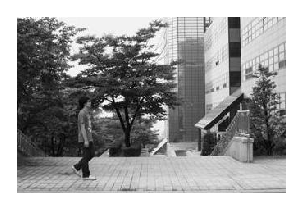
\includegraphics[width=0.23\textwidth]{paper-fig/fig20-2}}\hfill
  \subfigure[ ]{
\includegraphics[width=0.23\textwidth]{paper-fig/fig20-3}}
  \caption{Imbalance of background density. The first row illustrates a dynamic background image. There are swaying trees and small misalignments. The second row shows intensity distribution of the background in three different regions and straight lines are global thresholds. The third row represents detection result. Note that since other background subtraction methods try to classify foregrounds using a single threshold, false-positives are increased due to the imbalance among each background density.}
\end{figure}


Moreover, as dynamic backgrounds are varying frequently, the stationary background model based approaches generate many false-positives in those images due to the imbalance among each background density. (See figure 2). Thus, the background model should be extended to include nonstaionary backgrounds as normal. 
This paper presents the robust background model for containing dynamic backgrounds. In Section 2, the previous works and background works for the proposed method are discussed. 

The proposed work has two novel contributions: Firstly, the background is modeled on the shape-intensity joint domain, so it can estimate shape and intensity change simultaneously and improves discrimination compared to other intensity-based background models. Secondly, since background dynamics can be explained in the second-order space, we suggest the second-order background model for removing background’s variation. The suggested variation subtraction method generates stable response on dynamic background images and thus the threshold selection methods can be reliably applied to this model. In Section 3, 4, the suggested formulation and detailed algorithm is presented.

This method was tested on Natural scenes with dynamic background for object recognition and Semi-conductor wafer SEM images with noise for defect detection. The results show that the algorithm enhanced discrimination and successfully suppressed false-alarms from dynamic background. In Section 5, 6, detailed analysis and the experimental results are discussed, respectively.



\section{Related Work}

Background subtraction approaches can be categorized by their feature space. The first background subtraction methods [2, 3, 4] suggested statistical methods based on temporal consistency by assuming the single background modal. Single Gaussian [3] or median [4] was used for modeling background. Then, the mixture of Gaussians [5] was introduced for extending background model to the multi-modal. 

Non-parametric background model using kernel density estimation [6] was introduced. The rest of the background subtraction algorithms also have used kernel density estimation for measuring similarity between inspection data and training data. To find the probability that a point   belongs to training example  , an estimate can be computed as,
\begin{equation}
  1
\end{equation}
where h is a symmetric positive definite D × D bandwidth matrix. ‘’ denotes training example. The d-variate Gaussian function is a common choice as the kernel function K, 
\begin{equation}
  2
\end{equation}

The kernel function has a role in transforming the distance of   into the probability of their similarity. Then, the average probability of similarity is taken. The bandwidth h represents a generalization preference for decision. Data-driven bandwidth selection methods have been proposed, [18, 19].

Proximal neighborhoods’ smoothness assumption was considered for robustness of the likelihood. [6] used joint distribution among proximal neighborhoods. [7] tried discontinuity preserving smoothing for false-alarm suppression using graph-cut assuming the morphological smoothness.

Another attempt for robustness is that [7] suggested the likelihood ratio test between the background likelihood and the uniform distribution, so the likelihood values can be more stretched. [8] regarded proximal neighbors xc of x as single component and compared the component’s intensity histogram. The method showed the component consistency is more important than single pixel consistency. [9] estimated background density via variable bandwidth kernels for better data-driven estimation.

The attempts to deal with positional distribution were also introduced assuming that pixel positions can be changed in dynamic background. [6] corrected small misalignments by searching best correspondents in near positions. [7] incorporated position variable with temporal variable jointly. It searched best correspondence on entire positions for handling dynamic positional change.

[9] tried to combine another features into background model such as normalized color, and motion. They introduced motion information as a spatial relation parameter using optical flow assuming that intensity and optical flow features are uncorrelated. The result showed motion information is important for recognition. Consequently, the work implies that background density should be estimated based on both spatial and temporal domain.

  Background Variation Modeling approaches [10, 11] have been proposed. The background’s behavior was captured by given labeled motion images. Labeled motion images   are binary and acquired after simple background subtraction. Their main assumption is that the change of the binary motion label explains background’s behavior. Therefore, [10, 11] estimate the background variation by taking expectation of the classification rate from given labeled images. In the inspection stage, two subtractions are performed. The former is the simple background subtraction and the latter is the variation subtraction. Due to the second stage, varying backgrounds are classified to normal 

Shape matching algorithms define a shape as a gradient distribution with respect to space. The direct use of gradients is quite sensitive, so derivative of Gaussian (DoG) can be used in order to reduce noise effect, [13].
\begin{equation}
  3
\end{equation}
\begin{equation}
  4
\end{equation}
After separable convolution, Gx and Gy are obtained. [12, 14] commonly used log-polar coordinates for robust spatial representation. By transforming the (x, y) gradients in Cartesian coordinates into (θ, d) polar coordinates, a shape of each point is determined by two parameters, angle and distance respectively. Changing polar coordinates can be computed as,
\begin{equation}
  5
\end{equation}
\begin{equation}
  6
\end{equation}

The feature vector of the log-polar coordinates is defined as X ≡ (θ, log(|∇I|) ). The angle parameter θ indicates a shape of a point. The distance parameter log(|∇I|) captures a degree of flatness or edgeness. The log-scaled distance is used for reducing sensitiveness. Figure 3 represents Cartesian coordinates and log-polar coordinates. Note that flat regions only have small distances but they could have divergent angles among them due to the noise. In this case, the θ is meaningless, so it is desirable to set to θ = 0, if log(|∇I|) < 1. 

% \begin{figure}[t]
%   \centering
%   \label{fig30}
%   \subfigure[ ]{\includegraphics[width=0.15\textwidth]{paper-fig/fig30-1}}\hfill
%   \subfigure[ ]{\includegraphics[width=0.15\textwidth]{paper-fig/fig30-2}}
%   \caption{Log-polar Representation}
% \end{figure}

Shape matching algorithms find similar shapes by comparing spatial distribution among two local histograms. For measuring the spatial similarity,   test is commonly used, [14]:
\begin{equation}
  7
\end{equation}
  and   denote the K-bin normalized histogram at   and  , respectively. (7) is equivalent to the likelihood ratio test in [7, 11].



\section{Spatio-Temporal Consistency}
The suggested method considers spatial and temporal consistency jointly to estimate how much given inspection image is consistent with training examples. The spatial relation can be expressed by Shape distribution with respect to space. Also, the temporal relation can be represented by intensity distribution over time. Thus, the problem domain can be modeled in the structure of Spatio-Temporal Markov Random Field Model [1]. The proposed method is formulated based on the S-T MRF model.

Figure 4 shows the relation of Spatio-Temporal neighborhood on training image set. Each parallelogram represents a training image. A point   denotes (i, j) pixel on nth training image having x intensity. Subscript indicates temporal neighborhoods of x. Temporal consistency means that an intensity of a point   on inspection image should be statistically consistent with the intensities of  . 

Also,   represents spatial neighborhoods of  , such that  . Thus, the spatio-temporal consistency means that a component   should be statistically consistent with  . To avoid the curse of dimensionality, the spatial relation of   can be parameterized using gradients. Thus,   is equivalent to  . The spatio-temporal consistency can be represented by  . 

\begin{figure}[t]
  \centering
  \label{fig40}
  \subfigure[ ]{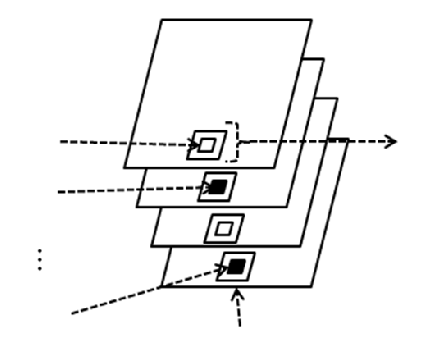
\includegraphics[width=0.15\textwidth]{paper-fig/fig40-1}}\hfill
  \subfigure[ ]{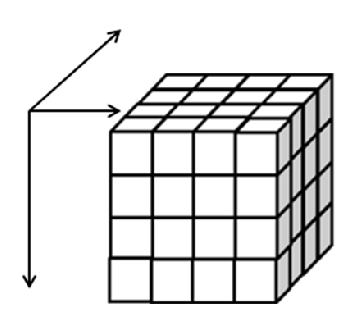
\includegraphics[width=0.15\textwidth]{paper-fig/fig40-2}}
  \caption{Spatio-Temporal Neighborhood}
\end{figure}


\subsection{Suggested Formulation}



\section{Spatio-Temporal Consistency}

\subsection{First-order Spatio-Temporal Background Model}

\subsection{Second-order Spatio-Temporal Background Model}



\section{Experimental Result}


\subsection{Application to Object Recognition of Dynamic scenes}

\subsection{Application to Defect Detection of Highly Noised SEM images}



\section{Discussion}





The foreground likelihood descriptor \begin{math} h_L(x) \end{math} and the expected likelihood descriptor
\begin{math} h_b(\hat{x}) \end{math} can be built from \begin{math} L(x), E(L(\hat{x})) \end{math} respectively.
The similarity of \begin{math} h_L(x) \end{math}  and \begin{math} h_b(\hat{x}) \end{math} can be obtained using 
\begin{math} \chi ^2 \end{math} test ( 7 ) and is called the second-order foreground likelihood \begin{math} L^2(x) \end{math}.
Also, the positional displacement within one pixel neighbors is considered using ( 12 ).

\ref{fig90} shows an example of variation subtraction process. (a), (b) represent \begin{math} E(\hat{L}) \end{math}.
(d), (g) indicates \begin{math} L \end{math}. (e), (h) are \begin{math} L^2 \end{math}.
By matching histograms between \begin{math} E(\hat{L}) \end{math} and \begin{math} L, L^2 \end{math} can be obtained.
Note that normal dynamic backgrounds are successfully suppressed close to 0, while keeping foregrounds' likelihood from being smoothed.








\bibliographystyle{ams[lain}
\bibliography{test}




\end{document}


